\documentclass[a4paper,10pt]{article}
\usepackage{My_math_package}

\title{MATH848G - Index Theory on Manifolds}
\author{Haoran Li}
\date{2019 Fall}

\makeindex[columns=2, title=Index, intoc] % Create the index

\begin{document}\sloppy % reduce overlong words

% Maketitle
\begin{titlepage}
\begin{center}
\vspace*{1cm}
\LARGE
\textbf{MATH848G - Index Theory on Manifolds} \\
\vspace{2cm}
\begin{center}
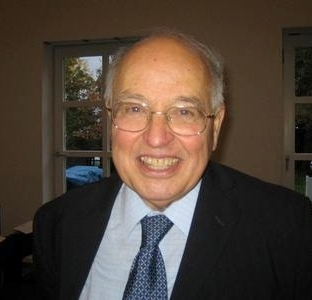
\includegraphics{Pictures/Michael_Francis_Atiyah.jpg}
\end{center}
\vspace{2cm}
\normalsize
Taught by \texttt{Jonathan Rosenberg} \\
Notes taken by \texttt{Haoran Li} \\
2019 Fall \\
\vspace{2cm}
Department of Mathematics\\
University of Maryland\\
\end{center}
\end{titlepage}

\tableofcontents
\newpage

\section{Pseudodifferential calculus}
\subfile{Pseudodifferential_calculus.tex}
\newpage

\section{K-theory}
\subfile{K-theory.tex}
\newpage

\section{Atiyah-Singer index theorem}
\subfile{Atiyah-Singer_index_theorem.tex}
\newpage

\section{Clifford algebra}
\subfile{Clifford_algebra.tex}
\newpage

\section{Spin group}
\subfile{Spin_group.tex}
\newpage

\begin{thebibliography}{}



\end{thebibliography}

\printindex
\newpage

\end{document}